\section{Transitoren}
	\subsection{Transistortypen}
	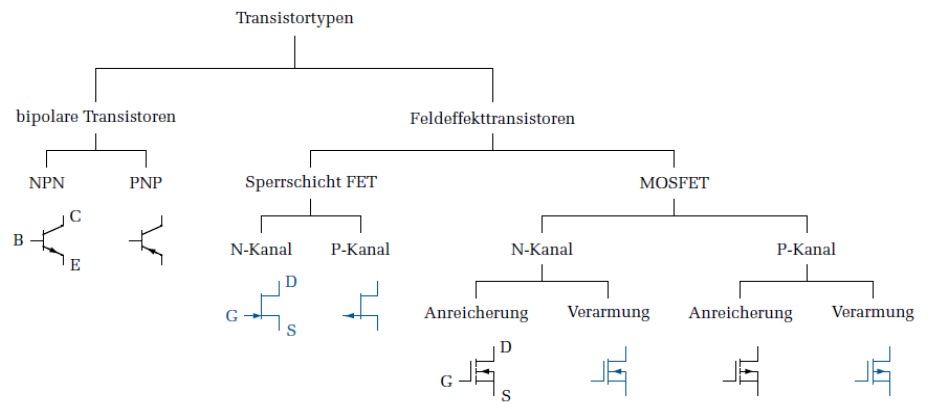
\includegraphics[width=11cm]{images/Transistortypen.png}

\subsection{Bipolartransistoren}
	\begin{minipage}[c]{6cm}
		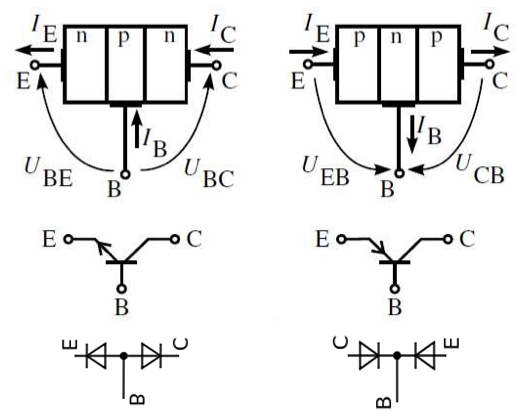
\includegraphics[width=6cm]{images/bipolarTransistor-Aufbau}
	\end{minipage}
	\begin{minipage}[c]{12cm}
		Links: NPN-Transistor \\
		Rechts: PNP-Transistor \\
		\\
		Die Schichten sind ungleich dick (Basis sehr dünn) und unterschiedlich dotiert.
		Sobald die BE-Diode Leitet, werden Elektronen vom Kollektor zur Basis gezogen und
		fliessen dann weiter zum Emitter. So steuert der Basisstrom $I_B$ den 
		Kollektorstrom $I_C$. \\
	\end{minipage} \\
	
	\begin{multicols}{2}
	\subsubsection{Betriebszustände}
		\begin{tabular}{l l}
			Normalbetrieb (Verstärker) & $V_{BE} > 0$, $V_{BC} < 0$\\
			Sättigung (Schalter EIN) & $V_{BE} > 0$, $V_{BC} > 0$\\
			Sperrbetrieb (Schalter AUS) & $V_{BE} < 0$, $V_{BC} < 0$\\
			Inversbetrieb (k. Anwendung) & $V_{BE} < 0$, $V_{BC} > 0$
		\end{tabular} \\
	\columnbreak
	\subsubsection{Stromverstärkungs-Faktoren}
		\begin{minipage}[c]{2.8cm}
			Basisschaltung \\
			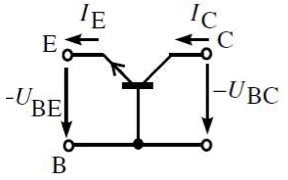
\includegraphics[width=2.8cm]{images/bip-basissch}\\
			$A_N=\frac{I_C}{I_E}$ \\
		\end{minipage}
		\begin{minipage}[c]{2.8cm}
			Emitterschaltung
			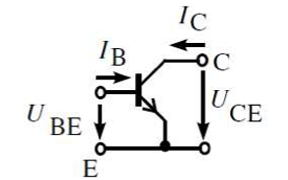
\includegraphics[width=2.8cm]{images/bip-emittersch}\\
			$B_N=\frac{I_C}{I_B}=\frac{A_N}{1-A_N}$ \\
		\end{minipage}
		\begin{minipage}[c]{2.8cm}
			Kollektorschaltung
			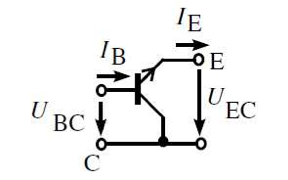
\includegraphics[width=2.8cm]{images/bip-kollektorsch}\\
			$C_N=\frac{I_E}{I_B}=\frac{1}{1-A_N}$ \\
		\end{minipage}
	\end{multicols}
	\subsubsection{Ebers-Moll-Modell}
		\begin{minipage}[c]{4cm}
			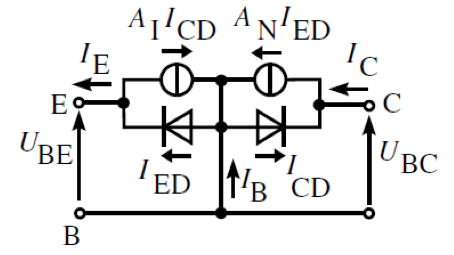
\includegraphics[width=4cm]{images/bipolar-EbersMoll}
		\end{minipage}
		\begin{minipage}[c]{8cm}
			$I_C=A_NI_{E_{sat}}(e^{\frac{U_{BE}}{U_T}}-1)
			 -I_{C_{sat}}(e^{\frac{U_{BC}}{U_T}}-1)$ \\
			$I_E=I_{E_{sat}}(e^{\frac{U_{BE}}{U_T}}-1)
			 -A_II_{C_{sat}}(e^{\frac{U_{BC}}{U_T}}-1)$ \\
			$I_B=I_E-I_C$ \\
		\end{minipage}
	
	\subsubsection{Kennlinien \& Formeln}
		\begin{minipage}[c]{4cm}
			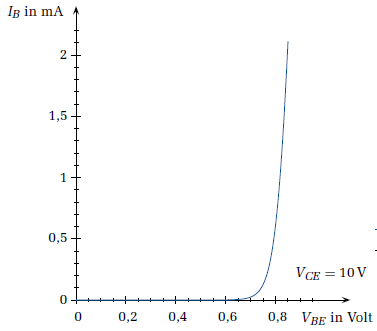
\includegraphics[width=4cm]{images/bipolarEingangsKennlinie}
		\end{minipage}
		\begin{minipage}[c]{5cm}
			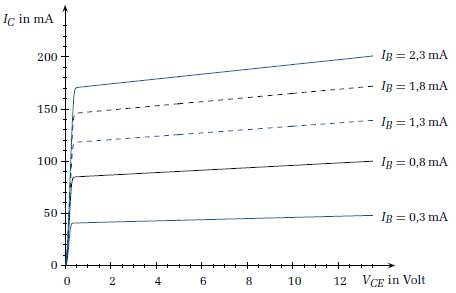
\includegraphics[width=5cm]{images/bipolarAusgangsKennlinie}\\
		\end{minipage}
		\begin{minipage}[c]{8cm}
			links: Eingangskennlinie - rechts: Ausgangskennlinie \\
			\\
			Kleinsignal-Widerstand: $r_{BE} = \frac{\delta V_{BE}}{\delta I_B} $ \\
			Basisstrom: $I_B=I_{B_{sat}}(e^{\frac{U_{BE}}{U_T}}-1)
						\approx I_{B_{sat}} e^{\frac{U_{BE}}{U_T}}$ \\
			Kollektorstrom: $I_C = B_N I_B+I_{CE_{0}} \approx B_N I_B$ \\
			
		\end{minipage}
	
	\subsubsection{Early-Effekt}
		\begin{minipage}[c]{5cm}
			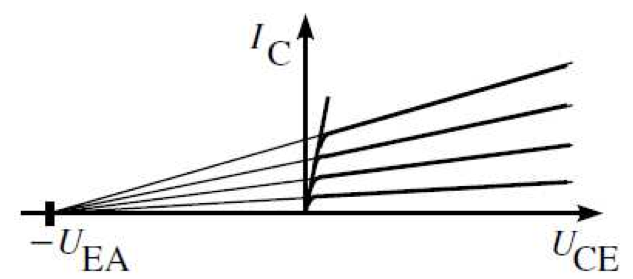
\includegraphics[width=5cm]{images/early-effekt}
		\end{minipage}
		\begin{minipage}[c]{12cm}
			Anstieg der Ausgangskennlinien beruht auf Veränderung der Basisweite infolge
			der Spannungsabhängigkeit der Sperrschichtweite der Basis-Kollektor-Diode. \\
			$U_{EA}$: Early-Spannung, Schnittpunkt der Ausgangskurven \\
			\\
			Modellerweiterung zur Berücksichtigung des Early-Effekts: \\
			$I_C = (B_NI_B+I_{CE_0})(1+\frac{U_{CE}}{U_{EA}}$
		\end{minipage}
		
	\subsubsection{Temperaturverhalten}
		Die maximale Leistung $P_V$ des Transistors muss stets kleiner als 
		$U_{CE} \cdot I_C$ sein. (Näherung) \\
		Zusätzlich muss die Wärme auch über das Gehäuse abgeführt werden können. Deshalb
		darf $P_V$ maximal $\frac{T_{max}-T_{amb}}{R_{th}}$ sein. ($R_{th}$: Thermischer
		Widerstand des Gehäuse) \\
		Der Transistor hat grundsätzlich das gleiche Temperaturverhalten wie die Diode. Somit
		gilt auch hier: $V_{BE}$ ändert um $-2\frac{mV}{K}$. Somit gilt für den
		Stromverstärkungsfaktor: $B_N=B_N(T_0)\cdot e^{C_b(T-T_0}$ mit 
		$C_b \approx 0.6\% \cdot K^{-1}$. Der hohe Temperatureinfluss muss bei der
		Schaltungsentwicklung berücksichtigt werden. \\
		
	\subsection{Kleinsignalverhalten}
		Beim Kleinsignal-Ersatzschaltbild wird das Verhalten des Transistors im Arbeitspunkt
		approximiert . Dazu wird ein Arbeitspunkt $AP$ im Kennlinienfeld eingezeichnet
		und dort linearisiert. \\
		\begin{minipage}[c]{6cm}
			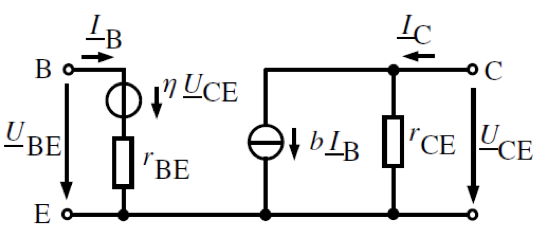
\includegraphics[width=6cm]{images/bip-kleinsignal}
		\end{minipage}
		\begin{minipage}[c]{6cm}
			$h_{11e} = r_{BE} = \frac{dU_{BE}}{dI_{B}} = \frac{U_T}{I_{B_0}}$ \\
			$h_{12e} = \eta = \frac{dU_{BE}}{dU_{CE}} \approx 0$ \\
			$h_{21e} = b = \frac{dI_C}{dI_B} = B_N(1+\frac{U_{CE_0}}{U_{EA}}) \approx B_N$ \\
			$h_{22e} = \frac{1}{r_{CE}} = \frac{dI_C}{dU_{CE}} = \frac{U_{EA}}{I_{C0}}$ \\
			$S = \frac{b}{r_{BE}}$
		\end{minipage}
		\begin{minipage}[c]{6cm}
			$r_{BE}$: Kleinsignal-Eingangswiderstand \\
			$\eta$: Kleinsignal-Spannungsrückwirkung \\
			$b$: Kleinsignal-Stromverstärkung \\
			$r_{CE}$: Kleinsignal-Ausgangswiderstand \\
			$S$: Kleinsignal-Steilheit
		\end{minipage} \\
		Kleinsignalmodell ohne Rückwirkung: $\eta \cdot U_{CE}$ wird weggelassen, weil 
		$\eta \approx 0$. Somit gilt: \\
		\begin{center}
			$\boxed{U_{BE} = r_{BE} \cdot I_B}$ \hspace{1cm} und \hspace{1cm}
			$\boxed{I_C = b \cdot I_B + \frac{1}{r_{CE}} \cdot U_{CE}}$ \\
		\end{center}
		
		Somit gilt für die \textbf{Emitterschaltung}: \\
		\begin{minipage}[c]{6cm}
			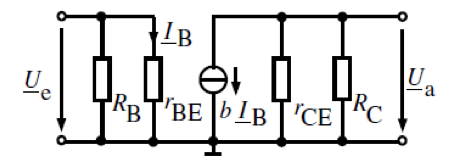
\includegraphics[width=6cm]{images/emittersch-esb}
		\end{minipage}
		\begin{minipage}[c]{12cm}
			$U_a = -b \cdot I_B \cdot (R_C || r_{CE})$ und $I_B=\frac{U_e}{r_{BE}}$ \\
			somit: $V_u = \frac{U_a}{U_e} = -\frac{b(R_C || r_{CE}}{r_{BE}}$ 
		\end{minipage} \\
		
	\subsection{Transistor als Schalter}
		